% =====================================================================
%  Guía de laboratorio — IEL04 — Circuitos Eléctricos I, semana 4
%  Escrita por src/guia_laboratorio.py con la plantilla institucional
%  (config/framework_iub/guia-laboratorio/: guialabiub.sty e img/, copiados a esta carpeta).
%
%  Compilar con:  pdflatex -> biber -> pdflatex -> pdflatex
%  (En Overleaf: compilador pdfLaTeX; biber se ejecuta solo.)
% =====================================================================
\documentclass[12pt]{article}

% Opciones: [sinmarca] quita la marca de agua; [borrador] muestra márgenes
%           [ieee] referencias IEEE (por defecto); [apa] referencias APA 7
\usepackage{guialabiub}

% ------- Tablas, diagramas de flujo, circuitos y gráficas (todo en LaTeX) -------
% (la plantilla no los trae; los estilos y la paleta son los del .tex del temario)
\usepackage{colortbl}                    % encabezado #121023 y filas alternas en las tablas
\usepackage{xltabular}                   % la tabla de materiales se parte entre páginas
\usepackage{tikz}
\usetikzlibrary{arrows.meta,positioning,shapes.geometric,shapes.misc}
\usepackage[siunitx,RPvoltages]{circuitikz}
\usepackage{pgfplots}
\pgfplotsset{compat=1.18}
\usepackage{adjustbox}

% Paleta del Manual de Identidad Visual IUB 2025 (los colores del manual y sus tintes)
\definecolor{iubnavy}{HTML}{121023}
\definecolor{iubyellow}{HTML}{FFDF2D}
\definecolor{iubwhite}{HTML}{FFFFFF}
\definecolor{iubblue}{HTML}{00ADE7}
\definecolor{iuborange}{HTML}{E39037}
\definecolor{iubgreen}{HTML}{3B9C6D}
\colorlet{iubgris}{iubnavy!18}
\colorlet{iubgrisoscuro}{iubnavy!60}
\colorlet{iubfondoazul}{iubblue!8}
\colorlet{iubfondonaranja}{iuborange!10}
\colorlet{iubfondoverde}{iubgreen!9}
\colorlet{iubfondogris}{iubnavy!5}
\colorlet{iubpurple}{iubnavy!45}
\pgfplotsset{cycle list={{iubblue, mark=*},{iuborange, mark=square*},{iubgreen, mark=triangle*},{iubnavy, mark=diamond*},{iubyellow, mark=pentagon*}}}

% Estilos de los diagramas de flujo (TikZ) y de las gráficas (pgfplots)
\tikzset{
  dcaja/.style={draw=iubblue, fill=iubfondoazul, line width=1pt, rounded corners=1pt, align=center, inner sep=2pt, text=iubnavy},
  destado/.style={draw=iubblue, fill=iubfondoazul, line width=1pt, rounded corners=6pt, align=center, inner sep=2pt, text=iubnavy},
  ddecision/.style={draw=iuborange, fill=iubfondonaranja, line width=1pt, diamond, aspect=1.6, align=center, inner sep=1pt, text=iubnavy},
  dterminal/.style={draw=iubgreen, fill=iubfondoverde, line width=1pt, rounded rectangle, align=center, inner sep=2pt, text=iubnavy},
  dflecha/.style={-{Stealth[length=2.4mm]}, line width=0.9pt, draw=iubnavy},
  drotulo/.style={font=\footnotesize, text=iubgrisoscuro, fill=white, fill opacity=0.92, text opacity=1, inner sep=1.5pt},
}
\pgfplotsset{iubejes/.style={width=0.9\linewidth, height=6.2cm, grid=major, grid style={iubgris}, axis lines*=left, axis line style={iubnavy}, tick label style={font=\small}, label style={font=\small}, title style={font=\bfseries\small}, legend cell align=left, legend style={draw=none, fill=none, font=\small, anchor=north, legend columns=-1, /tikz/every even column/.append style={column sep=8pt}}, unbounded coords=jump}}

% --------------------------- Bibliografía ----------------------------
\addbibresource{IEL04-semana04.bib}

% --------------------------- Datos de la guía -------------------------
\facultad{Facultad de Ingenierías}
\modulo{IEL04 --- Circuitos Eléctricos I}
\docente{Ing. Sergio Martinez Castilla}

\begin{document}

% Orden de la bibliografía: el mismo del .md (biblatex numera por orden de primera cita)
\nocite{ref1,ref2,ref3}

\datosguia
\lineablanco

% Título de la práctica y ficha de la sesión
{\centering\bfseries Guía de laboratorio: Circuito RC en serie: constante de tiempo con onda cuadrada y ley de voltajes de Kirchhoff en régimen sinusoidal\par}
\lineablanco
\textbf{Semana:} 4 de 14 \quad \textbf{Resultado de aprendizaje:} IEL04-RA2 \quad \textbf{Práctica:} propuesta a partir de la bibliografía \cite{ref1}, \cite{ref2}, \cite{ref3} \quad \textbf{Duración:} \SI{240}{\minute}
\lineablanco
La práctica corresponde a la sesión teórica de la semana 4, \guillemotleft{}El circuito RC en serie: carga del condensador, reactancia capacitiva, impedancia y ley de voltajes de Kirchhoff\guillemotright{}, y reproduce su caso de estudio: con el resistor de 1,5 k\ensuremath{\Omega} y el condensador C2 del kit se mide la constante de tiempo del circuito con una onda cuadrada y, con una señal sinusoidal de 1 kHz, las tensiones en el resistor y en el condensador, para verificar que su suma es fasorial y no aritmética. No hay un manual de laboratorio asignado al RA IEL04-RA2, por lo que la práctica se propone a partir de la bibliografía cargada: Floyd indica que para observar la carga y la descarga completas el semiperiodo de la onda cuadrada debe durar más de cinco constantes de tiempo y trata la ley de voltajes de Kirchhoff en circuitos RC \cite{ref1}; Boylestad desarrolla los transitorios de carga y descarga \cite{ref2} y Deorsola el régimen transitorio y la respuesta senoidal con fasores \cite{ref3}.

% ---------------------------------------------------------------------
\section{Objetivos}\label{sec:objetivos}
\textbf{Objetivo general:} Verificar experimentalmente la constante de tiempo y la ley de voltajes de Kirchhoff en un circuito RC en serie.
\lineablanco
\textbf{Objetivos específicos:}
\begin{itemize}
  \item Identificar por su marcado y verificar con instrumentos el resistor y el condensador del circuito. \emph{(CE1)}
  \item Medir las tensiones del resistor y del condensador con el multímetro de verdadero valor eficaz en régimen sinusoidal. \emph{(CE2)}
  \item Determinar experimentalmente la constante de tiempo y el ángulo de fase del circuito RC en serie con el osciloscopio, y comprobar la suma fasorial de tensiones. \emph{(CE3)}
\end{itemize}

% ---------------------------------------------------------------------
\section{Materiales y Equipos}\label{sec:materiales}
% --- Tabla: materiales y equipos (9; xltabular repite el encabezado si se parte) ---
\arrayrulecolor{iubnavy}
\begin{xltabular}{\linewidth}{>{\raggedleft\arraybackslash}p{0.6cm} >{\raggedright\arraybackslash}X >{\raggedright\arraybackslash}X >{\raggedleft\arraybackslash}p{2.2cm}}
\caption{Materiales y equipos de la práctica}\label{tab:materiales} \\
\rowcolor{iubnavy} \textcolor{white}{\textbf{\#}} & \textcolor{white}{\textbf{Material o equipo}} & \textcolor{white}{\textbf{Especificación}} & \textcolor{white}{\textbf{Cantidad}} \\
\endfirsthead
\rowcolor{iubnavy} \textcolor{white}{\textbf{\#}} & \textcolor{white}{\textbf{Material o equipo}} & \textcolor{white}{\textbf{Especificación}} & \textcolor{white}{\textbf{Cantidad}} \\
\endhead
\bottomrule
\endlastfoot
  1 & Resistor de película & 1,5 k\ensuremath{\Omega} \textpm{}5 \% (marrón-verde-rojo-oro) & 1 \\
  \rowcolor{iubfondogris} 2 & Condensador C2 del kit & 104K, 97,8 nF medidos & 1 \\
  3 & Generador de funciones & --- & 1 \\
  \rowcolor{iubfondogris} 4 & Osciloscopio de dos canales con puntas \texttimes{}10 & --- & 1 \\
  5 & Multímetro digital de verdadero valor eficaz & --- & 2 \\
  \rowcolor{iubfondogris} 6 & Medidor LCR & --- & 1 \\
  7 & Protoboard & --- & 1 \\
  \rowcolor{iubfondogris} 8 & Cables de conexión & --- & 12 \\
  9 & Resistencia de descarga & 1 k\ensuremath{\Omega} & 1 \\
\end{xltabular}

% ---------------------------------------------------------------------
\section{Procedimiento}\label{sec:procedimiento}
La práctica ocupa el bloque de 2 h de laboratorio de la sesión y se realiza en grupos de tres estudiantes, con tres roles que rotan entre etapas: quien monta y opera el circuito, quien mide y quien registra y verifica los cálculos. Antes de energizar cualquier montaje, el docente o el monitor revisa la conexión. Cada etapa abre con su diagrama de flujo, que muestra la secuencia y las comprobaciones de un vistazo, y sigue con sus pasos numerados; cada paso indica cuánto dura, qué debe observarse para saber que salió bien y qué hacer si no. Los valores numéricos de la sesión teórica sirven de referencia: las lecturas propias del grupo se registran en las tablas de la sección de análisis.
\lineablanco
% --- Etapa 1: Preparación y montaje (4 pasos) ---
\subsection{Preparación y montaje (\SI{19}{\minute})}\label{sec:etapa-1}
% --- Figura 1: diagrama de flujo de la etapa 1 (TikZ, con la paleta IUB) ---
\begin{figure}[H]
  \centering
\begin{adjustbox}{max width=\linewidth}
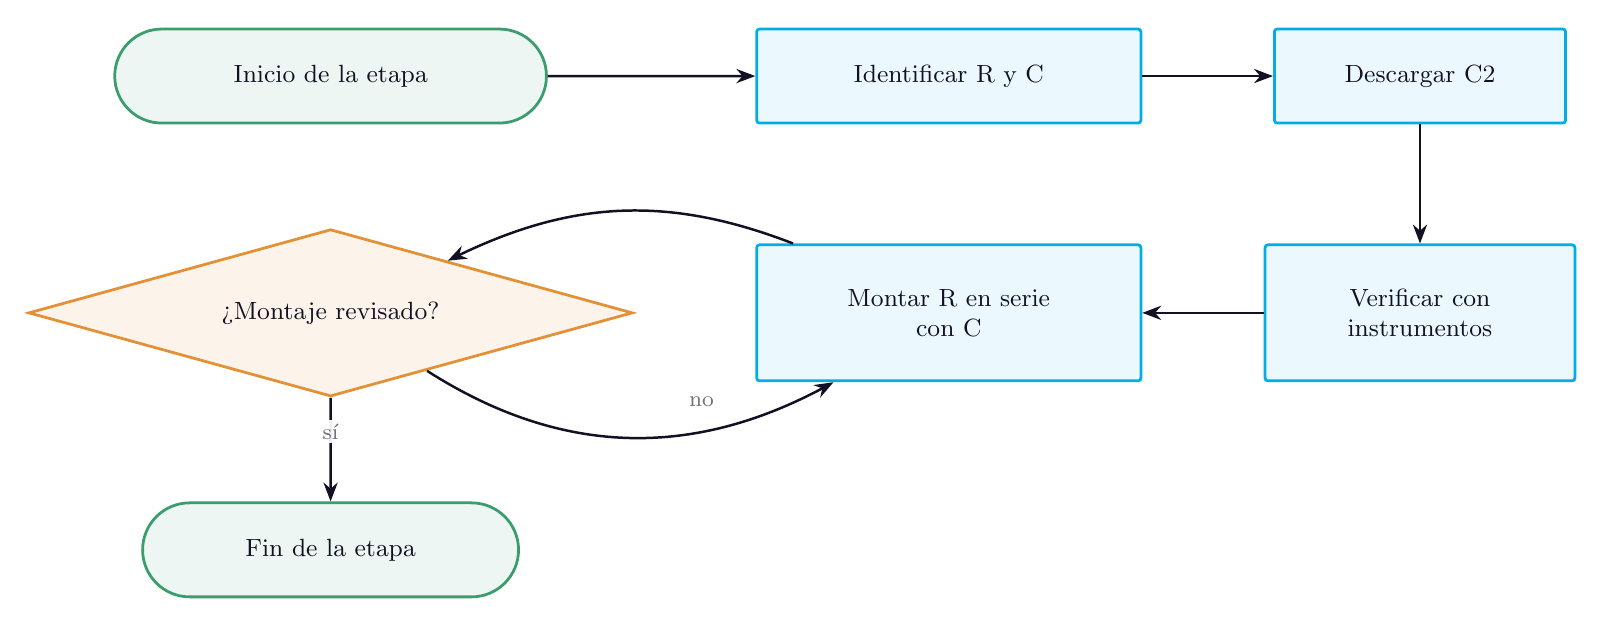
\begin{tikzpicture}[x=1in, y=1in, font=\small]
  % nodos (centro en pulgadas, con el tamano que calcula figuras.py)
  \node[dterminal, minimum width=2.214in, minimum height=0.470in] (n0) at (1.510,-0.235) {Inicio de la etapa};  % ini
  \node[dcaja, minimum width=1.921in, minimum height=0.470in] (n1) at (4.601,-0.235) {Identificar R y C};  % a0
  \node[dcaja, minimum width=1.456in, minimum height=0.470in] (n2) at (6.957,-0.235) {Descargar C2};  % a1
  \node[dcaja, minimum width=1.549in, minimum height=0.680in] (n3) at (6.957,-1.419) {Verificar con \\ instrumentos};  % a2
  \node[dcaja, minimum width=1.921in, minimum height=0.680in] (n4) at (4.601,-1.419) {Montar R en serie \\ con C};  % a3
  \node[ddecision, minimum width=3.021in, minimum height=0.799in] (n5) at (1.510,-1.419) {\textquestiondown{}Montaje revisado?};  % dec
  \node[dterminal, minimum width=1.935in, minimum height=0.470in] (n6) at (1.510,-2.604) {Fin de la etapa};  % fin
  % flechas (las de retorno, curvas)
  \draw[dflecha] (n0) -- (n1);
  \draw[dflecha] (n1) -- (n2);
  \draw[dflecha] (n2) -- (n3);
  \draw[dflecha] (n3) -- (n4);
  \draw[dflecha] (n4) to[bend right=24] (n5);
  \draw[dflecha] (n5) -- (n6);
  \draw[dflecha] (n5) to[bend right=31] (n4);
  % rotulos de las flechas (donde no caen sobre un nodo)
  \node[drotulo] at (1.510,-2.012) {sí};
  \node[drotulo] at (3.365,-1.865) {no};
\end{tikzpicture}
\end{adjustbox}
  \caption{Diagrama de flujo de la etapa 1: Preparación y montaje}
  \label{fig:flujo-1}
\end{figure}
\begin{pasos}
  \item \textbf{Paso~1:} Identificar el resistor por su código de colores (marrón-verde-rojo-oro: 1,5 k\ensuremath{\Omega} \textpm{}5 \%) \cite{ref1} y el condensador por su marcado (104K). \emph{(aprox.~\SI{4}{\minute})} \textbf{Comprobación:} Si el código leído no da 1,5 k\ensuremath{\Omega}, revisar el sentido de lectura empezando por la banda más cercana a un extremo.
  \item \textbf{Paso~2:} Descargar el condensador conectando entre sus terminales, durante unos segundos, una resistencia de 1 k\ensuremath{\Omega} sujeta con pinzas aisladas, y medir con el voltímetro en cd la tensión entre terminales. \emph{(aprox.~\SI{3}{\minute})} \textbf{Comprobación:} La tensión debe ser prácticamente nula (menos de 0,1 V); si no lo es, repetir la descarga antes de manipular el componente. \textbf{Seguridad:} No cortocircuitar los terminales con los dedos ni con una herramienta metálica: un condensador puede conservar carga después de desconectado.
  \item \textbf{Paso~3:} Verificar el resistor con el ohmímetro y el condensador C2 con el medidor LCR, y anotar sus valores medidos. \emph{(aprox.~\SI{6}{\minute})} \textbf{Comprobación:} El resistor debe leer cerca de 1492 \ensuremath{\Omega} y C2 cerca de 97,8 nF; si alguno sale de su tolerancia, reemplazarlo y anotar el nuevo valor.
  \item \textbf{Paso~4:} Montar en el protoboard el resistor en serie con C2, con el condensador del lado de tierra. \emph{(aprox.~\SI{6}{\minute})} \textbf{Comprobación:} El docente revisa el montaje antes de energizar. \textbf{Seguridad:} Montar con el generador apagado.
% figura del paso 4: Circuito RC en serie con el canal 2 del osciloscopio sobre el condensador (circuito en circuitikz)
\par\medskip\noindent
\begin{minipage}{\linewidth}
  \centering
  \begin{adjustbox}{max width=\linewidth}
    \begin{circuitikz}[color=iubnavy]
    \draw (0,0) to[sV, l=$v_s$] (0,3) to[R, l=$R$] (4,3) to[C, l_=$C_2$, v^=$v_C$] (4,0) -- (0,0); \draw (4,3) -- (6,3) to[voltmeter, l=CH2] (6,0) -- (4,0); \draw (0,0) node[ground]{};
    \end{circuitikz}
  \end{adjustbox}
  \captionof{figure}{Circuito RC en serie con el canal 2 del osciloscopio sobre el condensador}\label{fig:paso-4}
\end{minipage}
\par\medskip
\end{pasos}
% --- Etapa 2: Constante de tiempo con onda cuadrada (3 pasos) ---
\subsection{Constante de tiempo con onda cuadrada (\SI{19}{\minute})}\label{sec:etapa-2}
% --- Figura 3: diagrama de flujo de la etapa 2 (TikZ, con la paleta IUB) ---
\begin{figure}[H]
  \centering
\begin{adjustbox}{max width=\linewidth}
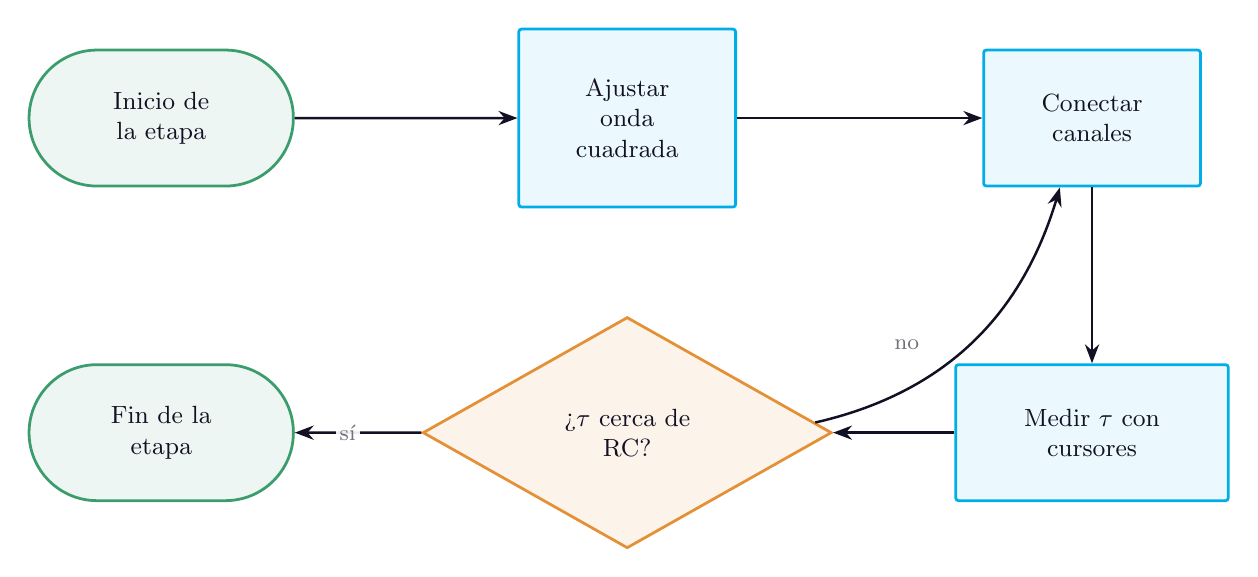
\begin{tikzpicture}[x=1in, y=1in, font=\small]
  % nodos (centro en pulgadas, con el tamano que calcula figuras.py)
  \node[dterminal, minimum width=1.377in, minimum height=0.680in] (n0) at (0.689,-0.445) {Inicio de \\ la etapa};  % ini
  \node[dcaja, minimum width=1.084in, minimum height=0.890in] (n1) at (3.019,-0.445) {Ajustar \\ onda \\ cuadrada};  % a0
  \node[dcaja, minimum width=1.084in, minimum height=0.680in] (n2) at (5.343,-0.445) {Conectar \\ canales};  % a1
  \node[dcaja, minimum width=1.363in, minimum height=0.680in] (n3) at (5.343,-2.018) {Medir \ensuremath{\tau} con \\ cursores};  % a2
  \node[ddecision, minimum width=2.045in, minimum height=1.156in] (n4) at (3.019,-2.018) {\textquestiondown{}\ensuremath{\tau} cerca de \\ RC?};  % dec
  \node[dterminal, minimum width=1.377in, minimum height=0.680in] (n5) at (0.689,-2.018) {Fin de la \\ etapa};  % fin
  % flechas (las de retorno, curvas)
  \draw[dflecha] (n0) -- (n1);
  \draw[dflecha] (n1) -- (n2);
  \draw[dflecha] (n2) -- (n3);
  \draw[dflecha] (n3) -- (n4);
  \draw[dflecha] (n4) -- (n5);
  \draw[dflecha] (n4) to[bend right=31] (n2);
  % rotulos de las flechas (donde no caen sobre un nodo)
  \node[drotulo] at (1.621,-2.018) {sí};
  \node[drotulo] at (4.417,-1.580) {no};
\end{tikzpicture}
\end{adjustbox}
  \caption{Diagrama de flujo de la etapa 2: Constante de tiempo con onda cuadrada}
  \label{fig:flujo-2}
\end{figure}
\begin{pasos}
  \item \textbf{Paso~5:} Ajustar el generador a una onda cuadrada de 0 V a 5 V y 500 Hz, de modo que el semiperiodo (1 ms) supere cinco constantes de tiempo (unos 750 \textmu{}s) \cite{ref1}. \emph{(aprox.~\SI{6}{\minute})} \textbf{Comprobación:} En el canal 1 debe verse la onda cuadrada de 5 V; si no, revisar la configuración del generador.
  \item \textbf{Paso~6:} Conectar el canal 1 a la salida del generador y el canal 2 sobre el condensador, con las puntas \texttimes{}10 compensadas y las tierras en el mismo nodo. \emph{(aprox.~\SI{5}{\minute})} \textbf{Comprobación:} En el canal 2 debe verse la curva exponencial de carga y descarga que llega a la meseta antes del flanco siguiente.
  \item \textbf{Paso~7:} Medir con los cursores de tiempo el intervalo entre el flanco de subida y el instante en que $v_C$ alcanza el 63,2 \% de su valor final; anotarlo como $\tau$ medida. \emph{(aprox.~\SI{8}{\minute})} \textbf{Comprobación:} El valor debe estar cerca de $\tau = RC$ calculada con los valores medidos (unos 146 \textmu{}s); si difiere más del 10 \%, revisar la escala de tiempo.
% figura del paso 7: Carga esperada del condensador con R = 1492 Ω y C = 97,8 nF (τ ≈ 146 µs) (gráfica en pgfplots con los puntos de su especificación)
\par\medskip\noindent
\begin{minipage}{\linewidth}
  \centering
  \begin{adjustbox}{max width=\linewidth}
    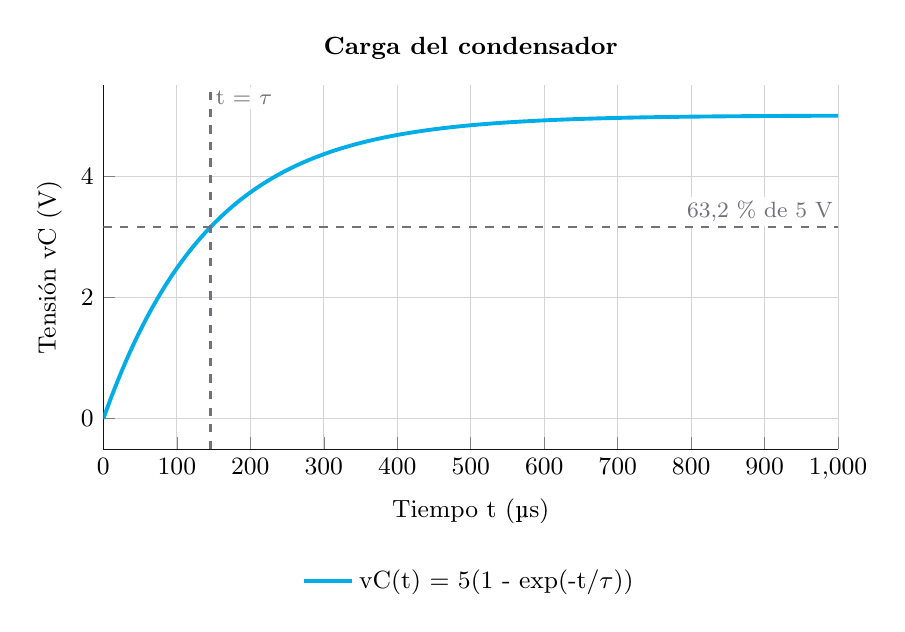
\begin{tikzpicture}
      \begin{axis}[
          iubejes,
          xlabel={Tiempo t (\textmu{}s)},
          ylabel={Tensión vC (V)},
          title={Carga del condensador},
          legend style={at={(0.5,-0.30)}},
          xmin=0,
          xmax=1000]
        % serie 1: vC(t) = 5(1 - exp(-t/τ)) («5*(1-exp(-t/tau))» en 300 puntos)
        \addplot[color=iubblue, line width=1.4pt, no markers] coordinates {
          (0,0) (3.34448,0.113312) (6.68896,0.224056) (10.0334,0.33229) (13.3779,0.438071) (16.7224,0.541456)
          (20.0669,0.642497) (23.4114,0.741248) (26.7559,0.837761) (30.1003,0.932088) (33.4448,1.02428) (36.7893,1.11438)
          (40.1338,1.20243) (43.4783,1.28849) (46.8227,1.37261) (50.1672,1.45481) (53.5117,1.53515) (56.8562,1.61368)
          (60.2007,1.69042) (63.5452,1.76542) (66.8896,1.83872) (70.2341,1.91037) (73.5786,1.98038) (76.9231,2.04882)
          (80.2676,2.1157) (83.612,2.18106) (86.9565,2.24495) (90.301,2.30738) (93.6455,2.3684) (96.99,2.42804)
          (100.334,2.48633) (103.679,2.54329) (107.023,2.59897) (110.368,2.65338) (113.712,2.70656) (117.057,2.75854)
          (120.401,2.80933) (123.746,2.85898) (127.09,2.9075) (130.435,2.95492) (133.779,3.00127) (137.124,3.04656)
          (140.468,3.09083) (143.813,3.1341) (147.157,3.17638) (150.502,3.21771) (153.846,3.2581) (157.191,3.29758)
          (160.535,3.33616) (163.88,3.37387) (167.224,3.41072) (170.569,3.44673) (173.913,3.48194) (177.258,3.51634)
          (180.602,3.54996) (183.946,3.58282) (187.291,3.61494) (190.635,3.64633) (193.98,3.67701) (197.324,3.70699)
          (200.669,3.73629) (204.013,3.76493) (207.358,3.79292) (210.702,3.82027) (214.047,3.84701) (217.391,3.87314)
          (220.736,3.89868) (224.08,3.92364) (227.425,3.94803) (230.769,3.97187) (234.114,3.99517) (237.458,4.01794)
          (240.803,4.0402) (244.147,4.06195) (247.492,4.08321) (250.836,4.10398) (254.181,4.12429) (257.525,4.14413)
          (260.87,4.16353) (264.214,4.18249) (267.559,4.20101) (270.903,4.21912) (274.247,4.23682) (277.592,4.25411)
          (280.936,4.27102) (284.281,4.28754) (287.625,4.30368) (290.97,4.31946) (294.314,4.33489) (297.659,4.34996)
          (301.003,4.36469) (304.348,4.37909) (307.692,4.39316) (311.037,4.40691) (314.381,4.42035) (317.726,4.43349)
          (321.07,4.44633) (324.415,4.45887) (327.759,4.47114) (331.104,4.48312) (334.448,4.49484) (337.793,4.50628)
          (341.137,4.51747) (344.482,4.52841) (347.826,4.5391) (351.171,4.54954) (354.515,4.55975) (357.86,4.56973)
          (361.204,4.57948) (364.548,4.58901) (367.893,4.59832) (371.237,4.60742) (374.582,4.61632) (377.926,4.62502)
          (381.271,4.63351) (384.615,4.64182) (387.96,4.64994) (391.304,4.65787) (394.649,4.66562) (397.993,4.6732)
          (401.338,4.68061) (404.682,4.68785) (408.027,4.69492) (411.371,4.70183) (414.716,4.70859) (418.06,4.7152)
          (421.405,4.72165) (424.749,4.72796) (428.094,4.73412) (431.438,4.74015) (434.783,4.74604) (438.127,4.75179)
          (441.472,4.75742) (444.816,4.76291) (448.161,4.76829) (451.505,4.77354) (454.849,4.77867) (458.194,4.78369)
          (461.538,4.78859) (464.883,4.79338) (468.227,4.79806) (471.572,4.80264) (474.916,4.80711) (478.261,4.81148)
          (481.605,4.81576) (484.95,4.81993) (488.294,4.82401) (491.639,4.828) (494.983,4.8319) (498.328,4.83571)
          (501.672,4.83943) (505.017,4.84307) (508.361,4.84663) (511.706,4.8501) (515.05,4.8535) (518.395,4.85682)
          (521.739,4.86006) (525.084,4.86323) (528.428,4.86633) (531.773,4.86936) (535.117,4.87232) (538.462,4.87522)
          (541.806,4.87805) (545.151,4.88081) (548.495,4.88351) (551.839,4.88615) (555.184,4.88873) (558.528,4.89125)
          (561.873,4.89372) (565.217,4.89613) (568.562,4.89848) (571.906,4.90078) (575.251,4.90303) (578.595,4.90523)
          (581.94,4.90737) (585.284,4.90947) (588.629,4.91152) (591.973,4.91353) (595.318,4.91549) (598.662,4.9174)
          (602.007,4.91928) (605.351,4.92111) (608.696,4.92289) (612.04,4.92464) (615.385,4.92635) (618.729,4.92802)
          (622.074,4.92965) (625.418,4.93124) (628.763,4.9328) (632.107,4.93432) (635.452,4.93581) (638.796,4.93727)
          (642.14,4.93869) (645.485,4.94008) (648.829,4.94144) (652.174,4.94276) (655.518,4.94406) (658.863,4.94533)
          (662.207,4.94657) (665.552,4.94778) (668.896,4.94896) (672.241,4.95012) (675.585,4.95125) (678.93,4.95235)
          (682.274,4.95343) (685.619,4.95449) (688.963,4.95552) (692.308,4.95653) (695.652,4.95751) (698.997,4.95848)
          (702.341,4.95942) (705.686,4.96034) (709.03,4.96124) (712.375,4.96211) (715.719,4.96297) (719.064,4.96381)
          (722.408,4.96463) (725.753,4.96543) (729.097,4.96622) (732.441,4.96698) (735.786,4.96773) (739.13,4.96846)
          (742.475,4.96918) (745.819,4.96988) (749.164,4.97056) (752.508,4.97123) (755.853,4.97188) (759.197,4.97251)
          (762.542,4.97314) (765.886,4.97375) (769.231,4.97434) (772.575,4.97492) (775.92,4.97549) (779.264,4.97605)
          (782.609,4.97659) (785.953,4.97712) (789.298,4.97764) (792.642,4.97815) (795.987,4.97864) (799.331,4.97912)
          (802.676,4.9796) (806.02,4.98006) (809.365,4.98051) (812.709,4.98095) (816.054,4.98139) (819.398,4.98181)
          (822.742,4.98222) (826.087,4.98262) (829.431,4.98302) (832.776,4.9834) (836.12,4.98378) (839.465,4.98414)
          (842.809,4.9845) (846.154,4.98486) (849.498,4.9852) (852.843,4.98553) (856.187,4.98586) (859.532,4.98618)
          (862.876,4.9865) (866.221,4.9868) (869.565,4.9871) (872.91,4.98739) (876.254,4.98768) (879.599,4.98796)
          (882.943,4.98823) (886.288,4.9885) (889.632,4.98876) (892.977,4.98901) (896.321,4.98926) (899.666,4.98951)
          (903.01,4.98974) (906.355,4.98998) (909.699,4.9902) (913.043,4.99042) (916.388,4.99064) (919.732,4.99085)
          (923.077,4.99106) (926.421,4.99126) (929.766,4.99146) (933.11,4.99166) (936.455,4.99184) (939.799,4.99203)
          (943.144,4.99221) (946.488,4.99239) (949.833,4.99256) (953.177,4.99273) (956.522,4.99289) (959.866,4.99305)
          (963.211,4.99321) (966.555,4.99336) (969.9,4.99352) (973.244,4.99366) (976.589,4.99381) (979.933,4.99395)
          (983.278,4.99408) (986.622,4.99422) (989.967,4.99435) (993.311,4.99448) (996.656,4.9946) (1000,4.99472)
        };
        \addlegendentry{vC(t) = 5(1 - exp(-t/\ensuremath{\tau}))}
        % línea de referencia en x = 145.9
        \draw[iubgrisoscuro, dashed, line width=0.9pt] ({axis cs:145.9,0}|-{rel axis cs:0,0}) -- ({axis cs:145.9,0}|-{rel axis cs:0,1}) node[drotulo, pos=1, anchor=north west] {t = \ensuremath{\tau}};
        % línea de referencia en y = 3.16
        \draw[iubgrisoscuro, dashed, line width=0.9pt] ({rel axis cs:0,0}|-{axis cs:0,3.16}) -- ({rel axis cs:1,0}|-{axis cs:0,3.16}) node[drotulo, pos=1, anchor=south east] {63,2 \% de 5 V};
      \end{axis}
    \end{tikzpicture}
  \end{adjustbox}
  \captionof{figure}{Carga esperada del condensador con R = 1492 \ensuremath{\Omega} y C = 97,8 nF (\ensuremath{\tau} \ensuremath{\approx} 146 \textmu{}s)}\label{fig:paso-7}
\end{minipage}
\par\medskip
\end{pasos}
% --- Etapa 3: Tensiones en régimen sinusoidal (4 pasos) ---
\subsection{Tensiones en régimen sinusoidal (\SI{29}{\minute})}\label{sec:etapa-3}
% --- Figura 5: diagrama de flujo de la etapa 3 (TikZ, con la paleta IUB) ---
\begin{figure}[H]
  \centering
\begin{adjustbox}{max width=\linewidth}
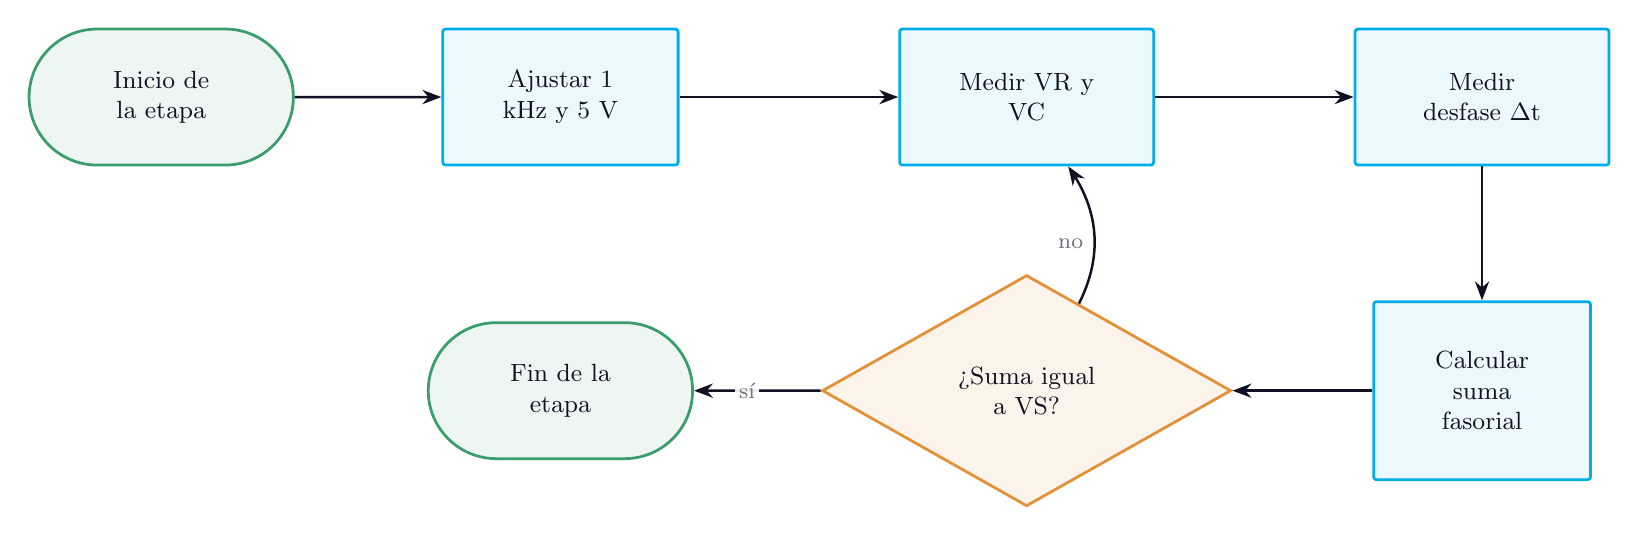
\begin{tikzpicture}[x=1in, y=1in, font=\small]
  % nodos (centro en pulgadas, con el tamano que calcula figuras.py)
  \node[dterminal, minimum width=1.377in, minimum height=0.680in] (n0) at (0.689,-0.340) {Inicio de \\ la etapa};  % ini
  \node[dcaja, minimum width=1.177in, minimum height=0.680in] (n1) at (2.685,-0.340) {Ajustar 1 \\ kHz y 5 V};  % a0
  \node[dcaja, minimum width=1.270in, minimum height=0.680in] (n2) at (5.016,-0.340) {Medir VR y \\ VC};  % a1
  \node[dcaja, minimum width=1.270in, minimum height=0.680in] (n3) at (7.293,-0.340) {Medir \\ desfase \ensuremath{\Delta}t};  % a2
  \node[dcaja, minimum width=1.084in, minimum height=0.890in] (n4) at (7.293,-1.808) {Calcular \\ suma \\ fasorial};  % a3
  \node[ddecision, minimum width=2.045in, minimum height=1.156in] (n5) at (5.016,-1.808) {\textquestiondown{}Suma igual \\ a VS?};  % dec
  \node[dterminal, minimum width=1.377in, minimum height=0.680in] (n6) at (2.685,-1.808) {Fin de la \\ etapa};  % fin
  % flechas (las de retorno, curvas)
  \draw[dflecha] (n0) -- (n1);
  \draw[dflecha] (n1) -- (n2);
  \draw[dflecha] (n2) -- (n3);
  \draw[dflecha] (n3) -- (n4);
  \draw[dflecha] (n4) -- (n5);
  \draw[dflecha] (n5) -- (n6);
  \draw[dflecha] (n5) to[bend right=31] (n2);
  % rotulos de las flechas (donde no caen sobre un nodo)
  \node[drotulo] at (3.618,-1.808) {sí};
  \node[drotulo] at (5.236,-1.074) {no};
\end{tikzpicture}
\end{adjustbox}
  \caption{Diagrama de flujo de la etapa 3: Tensiones en régimen sinusoidal}
  \label{fig:flujo-3}
\end{figure}
\begin{pasos}
  \item \textbf{Paso~8:} Ajustar el generador a una onda sinusoidal de 1 kHz y medir con el osciloscopio y con el multímetro de verdadero valor eficaz que la tensión en los bornes del circuito, con el circuito conectado, sea de 5,00 V eficaces. \emph{(aprox.~\SI{6}{\minute})} \textbf{Comprobación:} El multímetro debe indicar 5,00 V y el osciloscopio una sinusoide sin distorsión; si la tensión baja al conectar el circuito, reajustar la amplitud con el circuito conectado.
  \item \textbf{Paso~9:} Medir con el multímetro de verdadero valor eficaz la tensión en el resistor y la tensión en el condensador, y anotarlas. \emph{(aprox.~\SI{8}{\minute})} \textbf{Comprobación:} La suma aritmética de las dos lecturas debe superar 5 V; si da 5 V, revisar que el instrumento esté en ca.
  \item \textbf{Paso~10:} Con el canal 1 en la salida del generador y el canal 2 en el resistor, medir el desfase de tiempo $\Delta t$ entre los cruces por cero y calcular $\theta = 360^\circ \times f \times \Delta t$. \emph{(aprox.~\SI{10}{\minute})} \textbf{Comprobación:} El ángulo debe estar cerca de 47\textdegree{} de adelanto de la corriente; si sale mayor de 90\textdegree{}, revisar qué canal va adelantado.
  \item \textbf{Paso~11:} Calcular $\sqrt{V_R^2 + V_C^2}$ con las lecturas y compararlo con la tensión de la fuente. \emph{(aprox.~\SI{5}{\minute})} \textbf{Comprobación:} El resultado debe coincidir con 5,00 V a menos del 2 \%; si no, repetir las lecturas de tensión.
% ecuación del paso 11: Ley de voltajes de Kirchhoff en forma fasorial para el RC en serie:
\par Ley de voltajes de Kirchhoff en forma fasorial para el RC en serie:
\begin{equation}
  V_S = \sqrt{V_R^2 + V_C^2}
  \label{eq:paso-11}
\end{equation}
donde $V_S$, $V_R$ y $V_C$ son tensiones eficaces en voltios (V).
\end{pasos}
% --- Etapa 4: Desmontaje y cierre (3 pasos) ---
\subsection{Desmontaje y cierre (\SI{10}{\minute})}\label{sec:etapa-4}
% --- Figura 6: diagrama de flujo de la etapa 4 (TikZ, con la paleta IUB) ---
\begin{figure}[H]
  \centering
\begin{adjustbox}{max width=\linewidth}
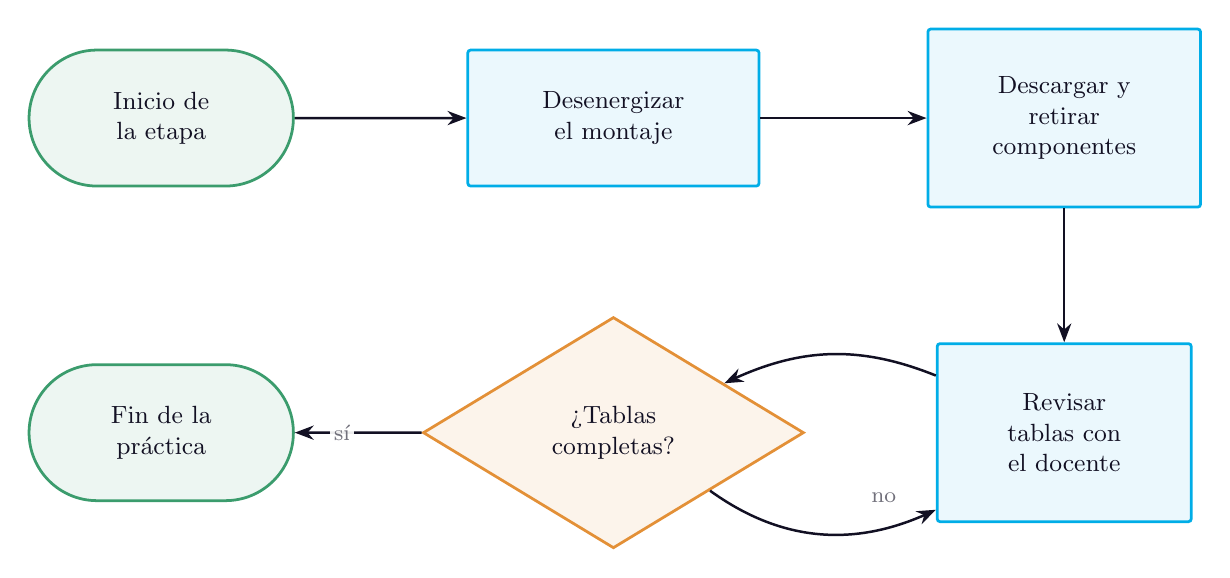
\begin{tikzpicture}[x=1in, y=1in, font=\small]
  % nodos (centro en pulgadas, con el tamano que calcula figuras.py)
  \node[dterminal, minimum width=1.377in, minimum height=0.680in] (n0) at (0.689,-0.445) {Inicio de \\ la etapa};  % ini
  \node[dcaja, minimum width=1.456in, minimum height=0.680in] (n1) at (2.950,-0.445) {Desenergizar \\ el montaje};  % a0
  \node[dcaja, minimum width=1.363in, minimum height=0.890in] (n2) at (5.204,-0.445) {Descargar y \\ retirar \\ componentes};  % a1
  \node[dcaja, minimum width=1.270in, minimum height=0.890in] (n3) at (5.204,-2.018) {Revisar \\ tablas con \\ el docente};  % a2
  \node[ddecision, minimum width=1.905in, minimum height=1.156in] (n4) at (2.950,-2.018) {\textquestiondown{}Tablas \\ completas?};  % dec
  \node[dterminal, minimum width=1.377in, minimum height=0.680in] (n5) at (0.689,-2.018) {Fin de la \\ práctica};  % fin
  % flechas (las de retorno, curvas)
  \draw[dflecha] (n0) -- (n1);
  \draw[dflecha] (n1) -- (n2);
  \draw[dflecha] (n2) -- (n3);
  \draw[dflecha] (n3) to[bend right=24] (n4);
  \draw[dflecha] (n4) -- (n5);
  \draw[dflecha] (n4) to[bend right=31] (n3);
  % rotulos de las flechas (donde no caen sobre un nodo)
  \node[drotulo] at (1.593,-2.018) {sí};
  \node[drotulo] at (4.302,-2.343) {no};
\end{tikzpicture}
\end{adjustbox}
  \caption{Diagrama de flujo de la etapa 4: Desmontaje y cierre}
  \label{fig:flujo-4}
\end{figure}
\begin{pasos}
  \item \textbf{Paso~12:} Apagar el generador de funciones y la fuente, desconectar las puntas del osciloscopio y retirar la alimentación del protoboard. \emph{(aprox.~\SI{3}{\minute})} \textbf{Comprobación:} Ningún indicador de salida debe quedar encendido en el generador ni en la fuente. \textbf{Seguridad:} Desenergizar siempre antes de retirar componentes.
  \item \textbf{Paso~13:} Descargar los condensadores del montaje con la resistencia de descarga, retirar los componentes y devolverlos al kit del grupo con su rótulo. \emph{(aprox.~\SI{4}{\minute})} \textbf{Comprobación:} El kit debe quedar completo, con cada componente en su lugar y con su valor medido anotado.
  \item \textbf{Paso~14:} Revisar con el docente las tablas de registro antes de abandonar el banco. \emph{(aprox.~\SI{3}{\minute})} \textbf{Comprobación:} Las tablas deben estar completas y con unidades; si falta un dato, repetir esa medición antes de desmontar el instrumento.
\end{pasos}

% ---------------------------------------------------------------------
\section{Cuestiones a Resolver}\label{sec:cuestiones}
\begin{enumerate}
  \item \textquestiondown{}Por qué el semiperiodo de la onda cuadrada debe superar cinco constantes de tiempo para medir \ensuremath{\tau}?
  \item \textquestiondown{}Qué diferencia porcentual hubo entre la \ensuremath{\tau} medida y la calculada, y qué elementos del montaje la explican?
  \item \textquestiondown{}Por qué la suma aritmética de VR y VC es mayor que la tensión de la fuente sin que se viole la ley de voltajes de Kirchhoff?
  \item \textquestiondown{}Qué ángulo de fase se obtuvo y cómo se compara con $\arctan(X_C/R)$ calculado con los valores medidos?
\end{enumerate}

% ---------------------------------------------------------------------
\section{Análisis de Resultados}\label{sec:analisis}
Calcular con los valores medidos de R y C la constante de tiempo, la reactancia $X_C = 1/(2\pi f C)$, la impedancia $Z = \sqrt{R^2 + X_C^2}$, la corriente y las tensiones esperadas, y compararlas con las mediciones en la tabla de registro, con su diferencia porcentual.
\lineablanco
Dibujar el diagrama fasorial de tensiones con las lecturas de VR y VC y el ángulo medido, y comprobar gráficamente que su suma vectorial reproduce la tensión de la fuente.
% --- Tabla de registro 1: Constante de tiempo del circuito RC en serie (3 filas vacías para registrar en el banco) ---
\begin{table}[H]
  \centering
  \caption{Constante de tiempo del circuito RC en serie}
  \label{tab:registro-1}
  \arrayrulecolor{iubnavy}
  \begin{tabularx}{\linewidth}{>{\raggedright\arraybackslash}X>{\raggedright\arraybackslash}X>{\raggedright\arraybackslash}X>{\raggedright\arraybackslash}X>{\raggedright\arraybackslash}X}
    \rowcolor{iubnavy} \textcolor{white}{\textbf{R medida (\ensuremath{\Omega})}} & \textcolor{white}{\textbf{C medida (nF)}} & \textcolor{white}{\textbf{\ensuremath{\tau} calculada (\textmu{}s)}} & \textcolor{white}{\textbf{\ensuremath{\tau} medida (\textmu{}s)}} & \textcolor{white}{\textbf{Diferencia (\%)}} \\
    \rule{0pt}{0.8cm} & & & & \\
    \rowcolor{iubfondogris} \rule{0pt}{0.8cm} & & & & \\
    \rule{0pt}{0.8cm} & & & & \\
    \bottomrule
  \end{tabularx}
\end{table}
% --- Tabla de registro 2: Tensiones y ángulo a 1 kHz (6 filas vacías para registrar en el banco) ---
\begin{table}[H]
  \centering
  \caption{Tensiones y ángulo a 1 kHz}
  \label{tab:registro-2}
  \arrayrulecolor{iubnavy}
  \begin{tabularx}{\linewidth}{>{\raggedright\arraybackslash}X>{\raggedright\arraybackslash}X>{\raggedright\arraybackslash}X>{\raggedright\arraybackslash}X>{\raggedright\arraybackslash}X}
    \rowcolor{iubnavy} \textcolor{white}{\textbf{Magnitud}} & \textcolor{white}{\textbf{Calculado}} & \textcolor{white}{\textbf{Medido}} & \textcolor{white}{\textbf{Unidad}} & \textcolor{white}{\textbf{Diferencia (\%)}} \\
    \rule{0pt}{0.8cm} & & & & \\
    \rowcolor{iubfondogris} \rule{0pt}{0.8cm} & & & & \\
    \rule{0pt}{0.8cm} & & & & \\
    \rowcolor{iubfondogris} \rule{0pt}{0.8cm} & & & & \\
    \rule{0pt}{0.8cm} & & & & \\
    \rowcolor{iubfondogris} \rule{0pt}{0.8cm} & & & & \\
    \bottomrule
  \end{tabularx}
\end{table}

% ---------------------------------------------------------------------
\section{Conclusiones}\label{sec:conclusiones}
Concluir si la constante de tiempo y las tensiones medidas concuerdan con el modelo del circuito RC en serie, explicando las diferencias con la resolución de los instrumentos y la resistencia interna del generador; relacionar la suma fasorial de tensiones con la ley de voltajes de Kirchhoff y con los criterios de medición del RA.
\lineablanco
\begin{itemize}
  \item \textquestiondown{}Qué tan bien coincidió \ensuremath{\tau} medida con el producto RC?
  \item \textquestiondown{}Qué demuestra la diferencia entre la suma aritmética y la fasorial de las tensiones?
  \item \textquestiondown{}Qué paso del procedimiento fue más sensible a errores de lectura?
\end{itemize}

% ---------------------------------------------------------------------
\section{Recomendaciones de Seguridad}\label{sec:seguridad}
\begin{itemize}
  \item Trabajar con el circuito desenergizado mientras se conecta o modifica el montaje; energizar solo después de la revisión del docente.
  \item Descargar los condensadores con una resistencia antes de manipularlos o medirlos, y respetar la polaridad de los electrolíticos: conectado con la polaridad invertida, un electrolítico puede explotar y provocar lesiones \cite{ref1}.
  \item Conectar las tierras de las dos puntas del osciloscopio a un mismo nodo de referencia: unirlas a nodos distintos cortocircuita el elemento que queda entre ellas.
  \item No superar la tensión de trabajo de C2 (100 V) ni la potencia del resistor; con 5 V de alimentación ambos trabajan holgados.
\end{itemize}

% ---------------------------------------------------------------------
\section{Bibliografía}\label{sec:bibliografia}
% Las fuentes cargadas se citan en el texto con \cite{refN}; el \nocite del principio fija su orden y \nocite{*} incluye las demás del .bib.
\nocite{*}
\bibliografia

\end{document}
